% !Mode:: "TeX:UTF-8"
%%% Local Variables:
%%% mode: latex
%%% TeX-master: t
%%% End:

\chapter{基于生成对抗网络的遥感影像分类方法}
\label{cha:chap03}

\section{引言}
%深度学习方法
深度学习模型组合低阶特征提取更加抽象、复杂的高阶特征,具有高效的特征学习能力,因而取代了传统的影像分类方法,成为当前遥感影像分类领域的主要研究方法。第~\ref{cha:chap02} 章概述了深度学习领域内重要的几个网络模型,并详细介绍了基于FCN 的遥感影像分类方法的结构和原理。一方面,FCN 中的卷积结构能自动学习输入图像的潜在特征;另一方面,FCN 反卷积结构将特征图恢复到原始图像尺寸,实现遥感影像的像素级分类。然而,FCN 模型上采样过程造成了特征信息的损失,导致网络预测地物边界模糊问题。此外,高分影像细节特征复杂且FCN 分割方法是影像像素点级的分类,使得预测结果中同类地物内部像素点难以保持类别一致性。进一步加剧了影像分类中地物边界模糊、歧义性等问题。


第~\ref{sec:chap02-3} 节介绍的GAN 模型是一个优秀的生成模型,其生成器和判别器不断对抗博弈,收敛时的GAN 模型生成器有强大的数据建模能力,判别器则会检测并纠正真实样本与生成数据之间的差异,保证整体的一致性。本章将对抗网络训练的思想引入到FCN 模型中,将FCN 模型像素级多分类交叉熵损失与GAN 对抗目标代价结合。对抗博弈中将促使分割模型生成的地物分类标签和真实地物Ground truth 图难以被判别器区分,从而提升同类地物内像素点类别的一致性。此外,对抗损失作用于整个影像数据,使得在几乎不增加模型复杂度的前提下提升影像远距离像素点间类别标签的连续性。


\section{基于CGAN 的影像分类方法}
\label{sec:firtst}

将对抗训练的思想应用到FCN 影像分类模型中,提升分类结果图中同类地物像素点的类别一致性。对抗网络的生成器需要预测原始影像的分割结果,这里原始影像作为先验条件输入对抗网络模型。因此,本章将有条件约束的对抗网络思想应用到FCN 影像分类模型中,提出基于CGAN 的遥感影像分类方法,其中原始影像作为CGAN 的先验约束条件。


\subsection{算法原理}
\label{subsec:firtst-1}
基于CGAN 的影像分类方法模型主要包含两个部分:生成网络的影像分割模型和对抗训练阶段的判别模型。整个模型结构如图\ref{fig:gan-fcn} 所示,左边是生成网络,是FCN 分割模型,其卷积特征提取结构使用VGGNet 16\cite{simonyan2014very}前五层的卷积结构,由五个卷积块堆叠而成,每个卷积块包含$2/3$个卷积层和$1$ 个最大池化层;分割模型的特征图恢复部分为$4$ 个反卷积的上采样结构,每个上采样模块中包含一次反卷积操作,将特征图尺寸放大两倍;最后通过一个$1\times 1$的卷积结构将特征图通道数降为1,生成影像分割结果。右边是判别网络,判别网络是一个二元CNN 分类模型,其输入存在两种情况:一种是原始影像和Ground truth 图拼接输入,另一种是原始影像与分割模型生成结果拼接输入。判别网络结构由两个卷积结构和两个全连接层堆叠,最后通过Sigmoid 激活函数判别当前输入样本来源,输出为一个二元分类值(输出为1代表它判断输入是第一种情况,输出为0代表它判断输入是第二种情况)。

\begin{figure}[htb]
  \centering
  \begin{center}
    \makebox[\textwidth]{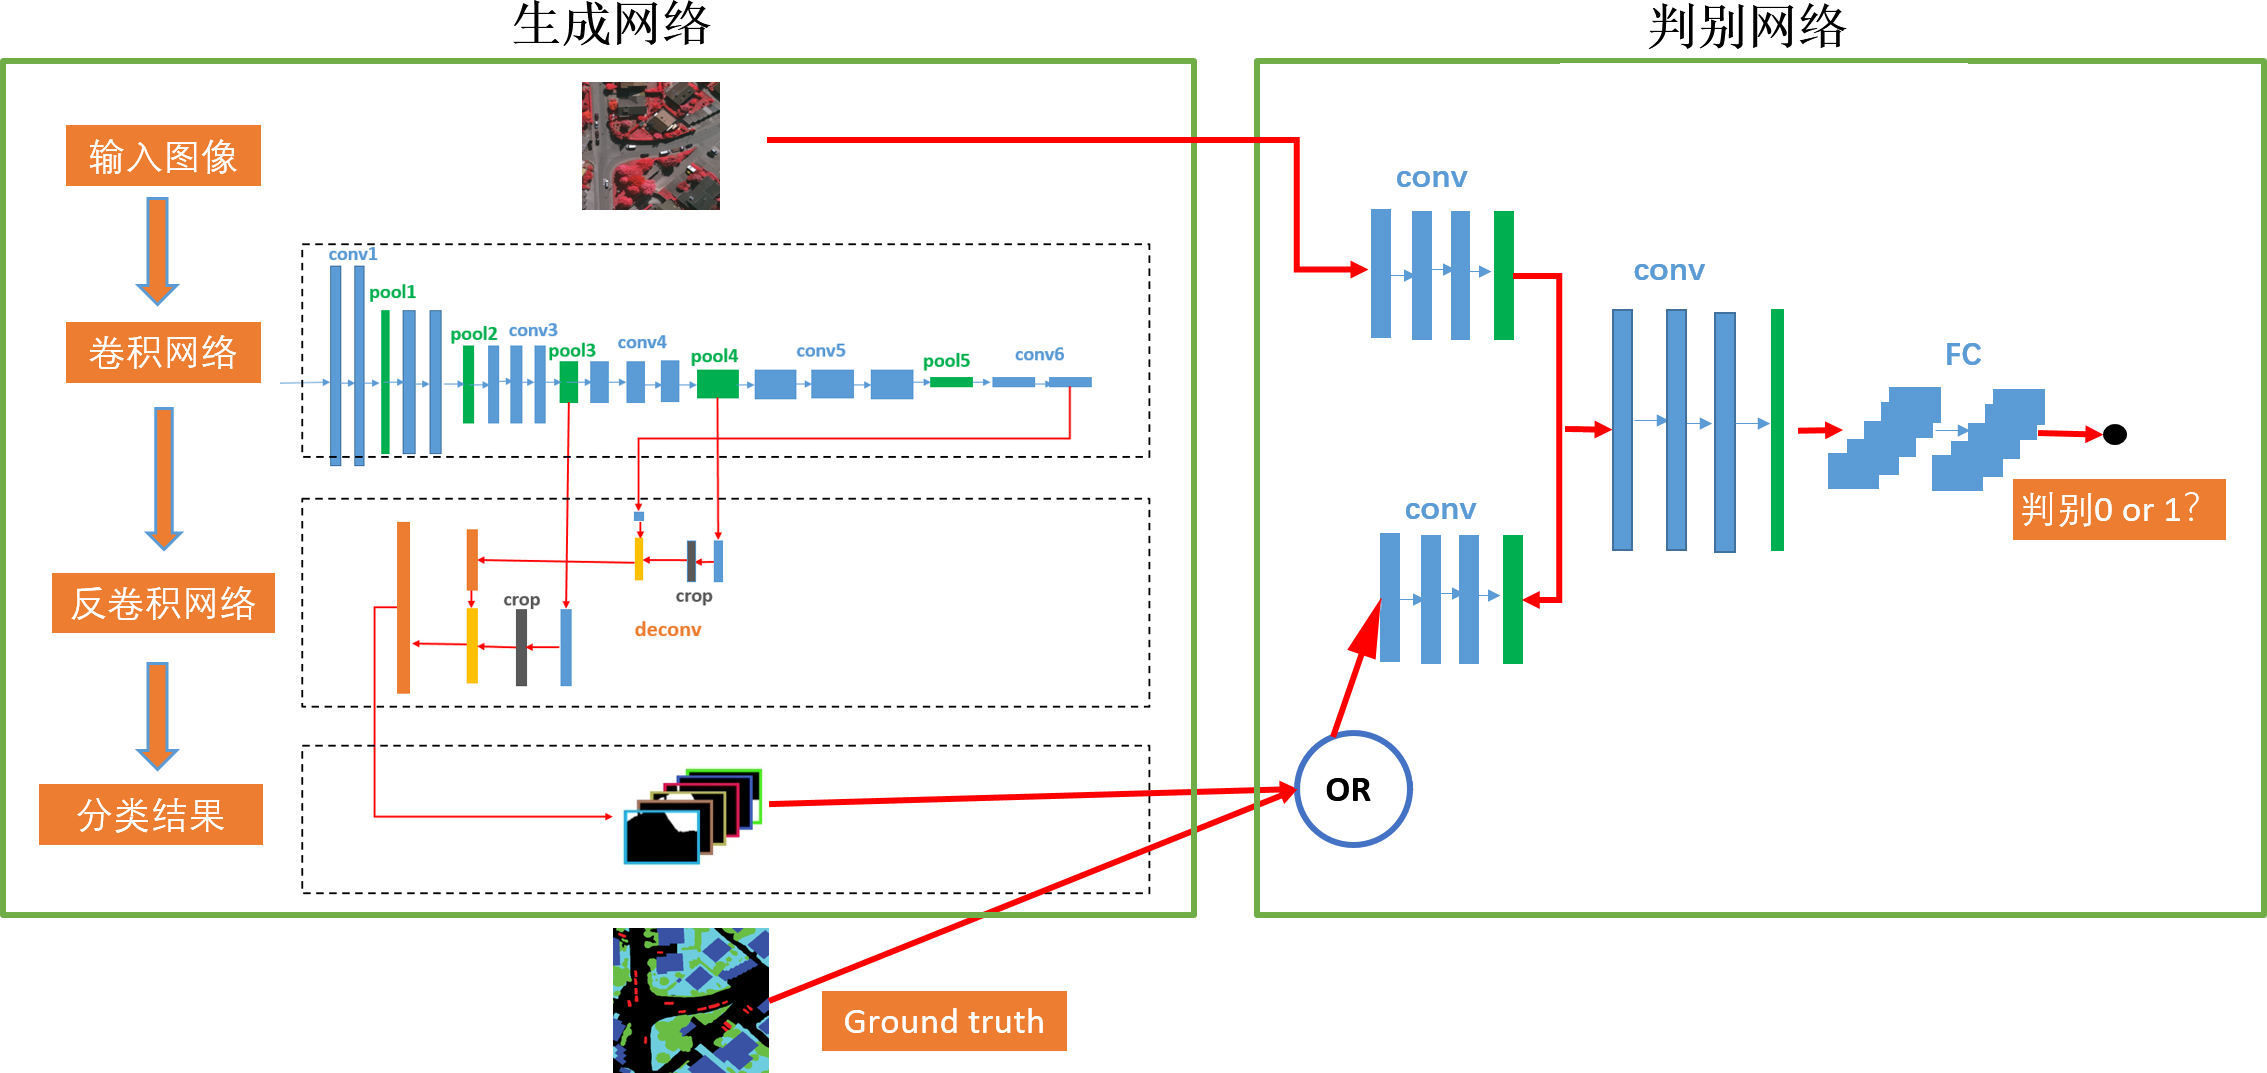
\includegraphics[width=\paperwidth]{figures/gan-fcn}}
    \caption{基于CGAN 的影像分类方法模型示意图}\label{fig:gan-fcn}
  \end{center}
\end{figure}

模型中使用二元分类损失(Binary classification loss, BCE)来度量判别网络。二元分类损失为二元交叉熵(cross entropy)函数,统计学中使用KL 散度衡量两个事件或分布中的不同,常用于计算代价损失,图像分类任务中最小化KL散度等价于最小化交叉熵,而交叉熵计算更简便\cite{de2005tutorial},因此文中用交叉熵来计算二元分类损失。交叉熵函数为分类预测概率值的负对数。二元交叉熵代价表达式如下:
\begin{equation}
  \label{eq:4-4}
  l_{bce} (\hat{z}, z) = -[z\log\hat{z} + (1-z)\log(1-\hat{z})]
\end{equation}

%+ (1-y_{ic})\log(1-\hat{y}_{ic})
生成网络是全卷积网络模型,其本质上是一个CNN 影像多分类模型。经典的多分类分割模型代价函数为多类别的交叉熵损失(multi-class entropy loss, MCE),分割模型输入为大小为$H\times W\times C$ 的图像,对图像做像素级预测分类,其多元交叉熵损失为:
\begin{equation}
  \label{eq:4-5}
  l_{mce} (\hat{y}, y) = -\sum_{i=1}^{H\times W}\sum_{c=1}^{C}y_{ic}\log\hat{y}_{ic}
\end{equation}
其中,$H$、$W$ 和$C$ 分别为图像的高度、宽度以及通道数。假定多分类问题中类标有$K$ 个取值,需要使用独热编码(One-hot encode)将图像类别标签编码为一个$K$ 维向量,借助Softmax 函数作为分类任务的输出层。Softmax 函数把神经网络分类输出转化为一组概率,且这组概率和为1。归属于类别$j$ 的概率为:
\begin{equation}
  \label{eq:4-6}
  p_j = \frac{e^{z_j}}{\sum_{k=1}^Ke^{z_k}}  \quad \forall j \in 1,2,\cdots, K
\end{equation}

假定有$N$ 张训练图片的数据集$X = \{x_1,x_2,\cdots, x_n \}$,对应的Ground truth 图标签集为$Y = \{y_1,y_2,\cdots, y_n \}$。输入图像大小为$H\times W\times C$(一般$C$ 取$3$),有$K$ 个类别的图像标签编码为$K$  维向量,即对第$i$ 张图像$x_i$,对应Ground truth 图有$y_j = [y_j^{(1)},y_j^{(2)}, \cdots, y_j^{(K)}]$。我们定义$g(x)$ 为输入图片$x$ 在生成网络分割模型下的预测输出,定义$d(x,y)\in [0,1]$ 为对抗网络判别图像标签$y$ 是输入图像$x$ 对应的Ground truth 图还是分割模型产生的分割结果的概率输出值。基于条件对抗网络框架的全卷积语义分割模型方法需要最小化分割模型的多分类交叉熵损失,同时最大化分割模型生成样本的判别概率。优化的目标代价函数为式\ref{eq:4-7}:
\begin{equation}
  \label{eq:4-7}
  L(\theta_g,\theta_d) = \sum_{n=1}^N \lbrace l_{mce} (g(x_n),y(n)) - \lambda [l_{bce} (d(x_n,y_n),1) + l_{bce}(d(x_n,g(x_n)),0)] \rbrace
\end{equation}
式中$\theta_g$ 和$\theta_d$ 分别代表分割模型和判别模型网络参数,右式中第一项为分割模型的交叉熵损失,第二项为对抗网络中样本判别损失代价函数,$\lambda$ 为生成阶段与对抗阶段代价权衡常数且有$\lambda > 0$。模型训练时我们需要最小化式\ref{eq:4-7} 中的代价函数,从而迭代求解得到网络参数$\theta_g$ 和$\theta_d$。

% 通过前向传播,利用最终分割模型对待分类测试影像求解每个像素属于各个类别的概率值
当模型迭代收敛后,模型中的权值参数均得以确定,此时模型中生成网络部分已经具有优秀的图像分割识别能力。通过前向传播,利用最终分割模型对待分类测试影像求解每个像素属于各个类别的概率值,像素点所属类别概率值求采用式\ref{eq:4-6} 中Softmax 函数求解,接着根据argmax 函数计算像素点最大概率值对应类别维度,即为当前预测点的分类标签,影像$x$ 上任一像素点$i$ 所属类别标签$C_k$ 的计算方式如式\ref{eq:4-8}。
\begin{equation}
  \label{eq:4-8}
  C_k = \mathop{\arg\max}_{k \in K} p_k(x^{(i)}), \ k=1,2,\cdots,K
\end{equation}
类似地,对待分类影像所有像素点预测类别标签,即可实现该影像的分割。

\subsection{算法实现}
\label{subsec:firtst-2}

基于CGAN 的遥感影像分类方法需要交替训练生成网络和判别网络两部分,算法采取小批次的随机梯度下降方法优化CGAN 权值参数,Adam \cite{kingma2014adam} 优化器可以自适应调整学习率的大小,因此本算法使用Adam 优化器更新模型权重。基于CGAN 的影像分类模型更新迭代伪代码如\textbf{算法~\ref{code:cgan}} 所示。

\begin{algorithm}[!h]
  \caption{基于CGAN 的遥感影像分类方法伪代码}
  \begin{algorithmic}[1]
    \Require
      原始影像$X$; 影像标签$Y$;
    \Ensure
      生成样本;

   \textbf{模型训练:}
    \State VGGNet16 前五层权值初始化生成模型,判别器步数 $k= 1$,权衡因子$\lambda$, 初始学习率$\alpha$, Adam 动量 $\beta_1,\beta_2$。
    \For{模型迭代epoch 数}
        \State \textbf{判别器:}
        \For{$k$ 步 }
        \State 小批次抽样$m$ 张影像$\{x^1,x^2,\cdots, x^m\}$; 对应影像的真实标签$\{y^1,y^2,\cdots, y^m\}$;这$m$ 张影像在生成器中的输出$\{g(x^1),g(x^2),\cdots, g(x^m) \}$
        \State 使用Adam 优化器更新判别器的权重:
        $$
        \nabla_{\theta_d} \frac{1}{m} \sum_{i=1} ^m [\log(d(x^i,y^i)) + \log(1-d(x^i,g(x^i)) ]
        $$
        \EndFor
        \State \textbf{生成器:}
        \State 小批次抽样$m$ 张影像$\{x^1,x^2,\cdots, x^m\}$;
        \State 分割模型输出这$m$ 张影像分割结果$\{g(x^1),g(x^2),\cdots, g(x^m) \}$
        \State 使用Adam 优化器更新生成器的权重:
        $$
        \nabla_{\theta_g} \frac{1}{m} \sum_{i=1} ^m [\log(1-d(x^i,g(x^i))]
        $$
    \EndFor

  \textbf{模型预测:}
    \State 模型迭代收敛后,用生成器分割模型对测试影像预测分割结果,采用概率最大化预测类别标签:
    $$
    C_k = \mathop{\arg\max}_{k \in K} p_k(x^{(i)}), \ k=1,2,\cdots,K
    $$
      
  \end{algorithmic}
  \label{code:cgan}
\end{algorithm}


模型首先将影像数据划分为训练集和测试集,并赋值给对应变量。初始化CGAN 分割模型的超参数。在每次迭代内,分批次随机抽取生成分割图和Ground truth 图,分别与对应的原始影像对应拼接,联合输入判别模型,计算判别模型损失并更新判别模型相关权值参数。接着固定判别模型训练生成网络,计算模型损失并更新生成器参数权重,完成网络的一次迭代。模型收敛后即用生成分割模型对测试集影像进行处理,得到模型分割结果图。


\section{实验数据介绍与预处理}
\label{sec:second}

\subsection{Vaihingen 数据介绍}
\label{sec:second-1}
本章实验数据源为ISPRS(国际摄影测量及遥感探测学会)提供的Vaihingen 高分辨率遥感影像数据\footnote{Vaihingen 数据集官网链接:http://www2.isprs.org/commissions/comm3/wg4/detection-and-reconstruction.html}。Vaihingen 数据集由德国测量和遥感协会(DGRF)于2010年使用空中数字摄像机拍摄,拍摄区域为半农村地区的德国斯图加特市法伊欣根市镇(Vaihingen),影像空间分辨率为$0.09m$。如图\ref{fig:vaihingen}(a) 所示为Vaihingen 数据整体图,整个数据被划分为33幅大小不一的图像,其中带有真实地面数据的影像为16幅。Vaihingen 数据包含三个波段(近红外-红-绿)的正射影像数据(Orthophoto)、数字地表模型(Digital Surface Model,DSM)数据以及拍摄区域真实地物分类结果(Ground truth)。图\ref{fig:vaihingen}(b-d) 分别为该影像某一区域的正射影像、DSM高程、Ground truth 图。

\begin{figure}[!htb]
  \centering
  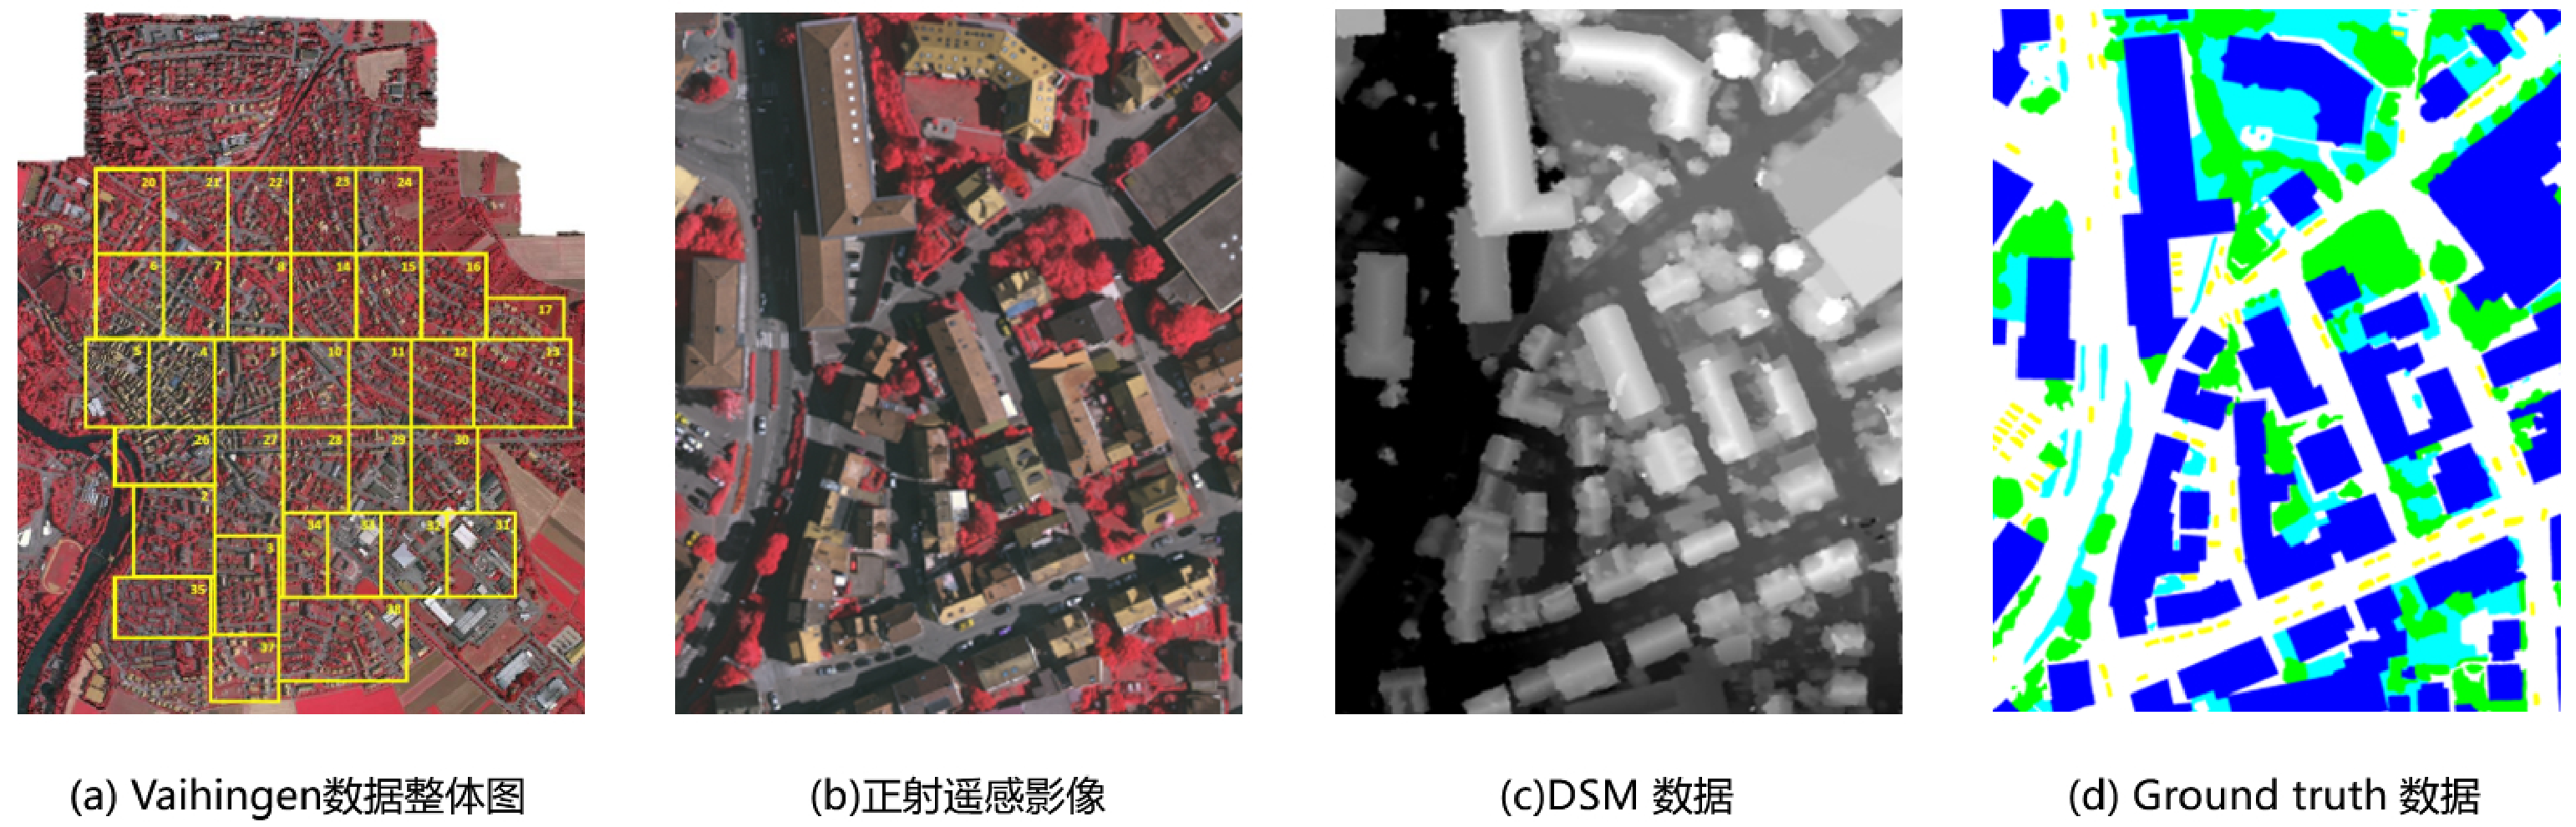
\includegraphics[width=0.98\textwidth]{figures/vaihingen2}
  \caption{Vaihingen 影像数据}\label{fig:vaihingen}
\end{figure}

Vaihingen 地区影像依据领域专家人工解译结果划分为地面、低矮植被、树木、建筑物、车辆、背景六类地物。Ground truth 图中六类地物的类别和对应颜色分别如表\ref{tab:vaih_gt} 所示。

\begin{table}[!htbp]
  \caption{Vaihingen 数据类别标签颜色对照表}\label{tab:vaih_gt}
  \centering
  \footnotesize

  \begin{tabular}{p{2cm}p{2cm}p{3cm}p{2cm}}
    \toprule
    地物类别 & 颜色 & 色彩值(R,G,B)   & 类别标签 \\
    \midrule
    地面     & 白色 & $(255,255,255)$ & 0        \\
    低矮植被 & 青色 & $(0,255,255)$   & 1        \\
    树木     & 绿色 & $(0,255,0)$     & 2        \\
    建筑物   & 蓝色 & $(0,0,255) $    & 3        \\
    车辆     & 黄色 & $(255,255,0)$   & 4        \\
    背景     & 红色 & $(255,0,0) $    & 5        \\
    \bottomrule
  \end{tabular}
\end{table}

\subsection{数据预处理}
\label{sec:second-2}

\subsubsection*{1. 波段组合}
Vaihingen 高分辨率影像空间、几何信息丰富,但正射影像光谱波段只有三个,仅使用正射影像数据无法完备有效地提取影像特征。而对于光谱相似区域的地物,如地面、建筑物、阴影等,更加难以区分,DSM 数据包含了地形、桥梁、房屋住宅和树木等高度地面高程信息,对模型区分地表建筑物、地面影像、不同高度植被一定程度上能提供帮助。Vaihingen 影像的DSM 包含一个波段,其像素值表示高度值。因此,将Vaihingen 数据的DSM 作为额外的波段附加在正射影像波段后,参与模型训练。

\subsubsection*{2. 数据集划分}
Vaihingen 数据中带有Ground truth 图的影像共有16张,实验中选取12张影像(标号为$1,5,7,11,15,17,21,26,28,30,32$ 和$37$)作为模型训练集,另外4张影像(标号为$3,13,23,34$)作为模型测试集。将影像Ground truth 图由RGB 图像转化为1维类别标签标签,各地物类别与对应的标签如表\ref{fig:vaihingen} 所示。

\subsubsection*{3. 数据归一化}
Vaihingen 影像数据集各通道的像素点取值在$[0,255]$ 范围内,像素点的分布范围较广,如果直接输入神经网络容易引起神经元输出因输入绝对值过大而饱和的现象,从而整个网络难以收敛。所以需要对图像数据做归一化处理,即将图像像素点取值从$[0,255]$ 范围映射到一个较小的变化范围,把有量纲表达式变为无量纲表达式,加快训练网络的收敛速度。

图像常用归一化方法有均值方差标准化和最大最小值归一化这两种。均值方差标准化又叫做z-score 标准化,其处理过程是原始数据与平均值的差再除以标准差。如式\ref{eq:4-9} 所示,
\begin{equation}
  \label{eq:4-9}
  z = \frac{x-\mu}{\sigma}
\end{equation}
式中$x$ 为原始输入数据,$\mu$ 和$\sigma$ 分别为数据的平均值和标准差,$z$ 为$x$ z-score 标准化后的输出。 经过z-score 标准化后数据服从均值为0、方差为1的正态分布,该方法多用于预处理没有明显边界的数据。

最大最小值归一化方法则是通过线性函数转换,将某变化范围内数据映射到$[0,1]$ 之间,线性映射过程如式\ref{eq:4-10} 所示:
\begin{equation}
  \label{eq:4-10}
  y = \frac{x-x_{min}}{x_{max}-x_{min}}
\end{equation}
式中$x$ 为原始输入数据,$x_{max}$ 和$x_{min}$ 分别为数据的最大值和最小值,$y$ 为$x$ 最大最小值归一化后的输出。

本实验中采用最大最小值归一化方法对高分影像做归一化处理,将影像像素值从$[0,255]$ 映射到$[0,1]$ 之间,加快神经网络的训练和收敛速度。

\subsubsection*{4. 样本选取与数据增强}
高分影像单张图像尺寸通常很大,直接送入神经网络计算量太大,无法完成训练。Vaihingen 单张影像尺寸大约为 $2563 \times 2049$,不能直接用于网络训练。本实验中对原始影像进行裁切处理,将影像裁剪为大小$256 \times 256$ 的图像块作为模型训练集样本。可有效降低网络训练计算量,避免内存溢出。

\begin{figure}[!htbp]
  \centering
  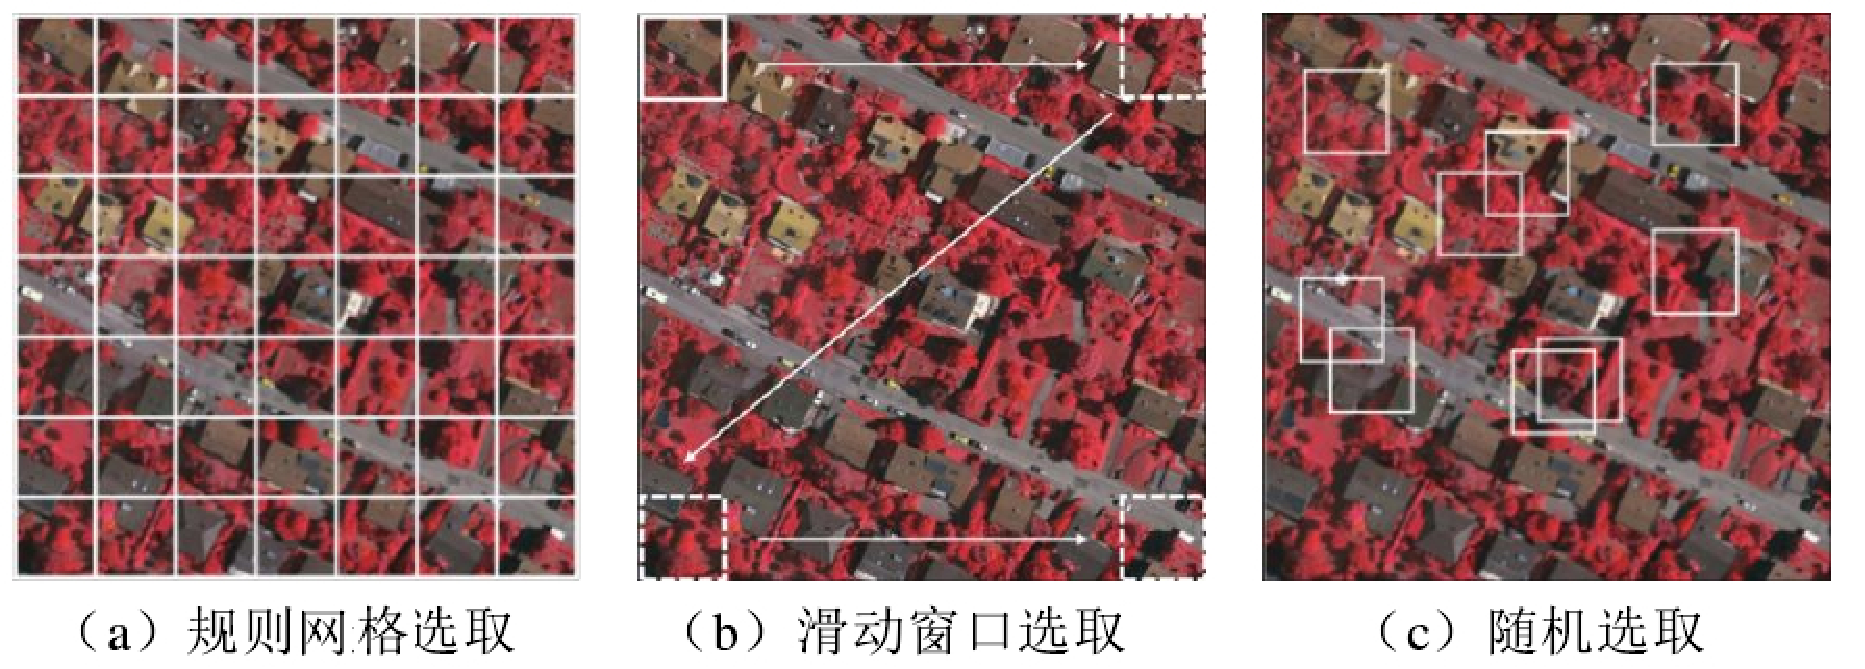
\includegraphics[width=0.8\textwidth]{figures/sample_data}
  \caption{图像裁剪方式}\label{fig:sample_data}
\end{figure}

常用图像裁剪方式有规则网格选取、滑动窗口裁剪和随机选取。规则网格选取是使用大小为$256 \times 256$ 的网格切分影像,这种划分方式得到的样本量有限。滑动窗口裁剪方法以特定的移动间隔在原始影像上剪裁得到训练样本。文中采用滑动窗口尺寸为$256 \times 256$,滑动窗口样本受滑动间隔尺度影像,滑动间隔小得到的冗余影像过多,滑动间隔大则会丢失影像许多特征信息。随机选取则是使用$256 \times 256$ 的裁剪窗口在原始影像上裁切获得样本。这种方法灵活便捷,能够有效利用遥感影像的信息,且裁剪出大量的训练样本。三种裁剪方式如图\ref{fig:sample_data} 所示。

本文实验中训练样本采用随机裁剪选取方式获得,测试样本采用规则网格选取方式获得。获取裁剪样本时也对同一区域的DSM、Ground truth 图数据进行裁切,保证输入数据与类别标签的一致性。

另外,为了获取更多的有效数据,增强网络模型的泛化能力,这里对训练样本做数据增强(Data augmentation)处理。数据增强是通过一些几何变换(如平移、旋转和翻转)从已有训练样本图像生成一些新的样本,来扩大训练数据集。文中对上一步裁剪获得的训练样本做镜像对称,水平翻转处理,来扩大已有训练样本集,增强模型泛化能力。

本小节对Vaihingen 有标签的16块影像数据处理,其中12张影像得到训练集样本图像$5760$ 幅,用于测试集的4 张影像经规则网格选取法得到大小为$256 \times 256$ 的测试图像合计$320$ 张。




\section{实验结果与分析}
\label{sec:third}
\subsection{实验环境}
\label{sec:third-1}
本章实验电脑为思腾合力IR4200 服务器,其主要参数如下:CPU 为两块 Intel Xeon E5-2690 2.9GHz 8核 16线程正式版处理器,内存为128G 容量8通道DDR4 服务器内存,GPU 为技嘉 1080Ti,显存 12G。实验中使用 Ubuntu 16.04 LTS 操作系统,编程语言为Python 3.5,神经网络模型采用谷歌开源框架Tensorflow 编程实现,Tensoflow 版本为1.5.0。

\subsection{评价指标}
\label{sec:third-2}
本节实验分别通过定性和定量两种指标来评估影像分割结果。定性即人工主观对测试图像的分割结果图做出评判,定量分析则使用图像分割中常用到的两种指标:

(1)总体精度(Overall accuracy,OA),即遥感影像分类精度最直观的评价指标,其值为影像中被正确分类的像元个数除以总像元个数,其计算方式如下式:
\begin{equation}
  \label{eq:4-11}
  OA = \frac{1}{A_{\mbox{总}}}  \sum_{k=1}^K a_{kk}
\end{equation}
式中$A_{\mbox{总}}$ 为真实地物像元总数,$K$ 为地物类别数,$a_{kk}$ 第$k$ 类地物被正确分类的像元数。

(2)平均交并比(Mean Intersection over union, mIoU),IoU 是影像中真实标签与预测分割结果两者交集与并集的比值,mIoU 是图像语义分割领域最常用的准确度度量方法,它分别对影像每个地物类别计算IoU,然后再对所有地物类别的IoU 求均值。IoU 的计算方式如式\ref{eq:4-12}:
\begin{equation}
  \label{eq:4-12}
  IoU = \frac{\mbox{预测结果} \cap \mbox{真实标签}}{\mbox{预测结果} \cup \mbox{真实标签}}
\end{equation}
影像所有类别地物的mIoU 的计算方式如式\ref{eq:4-13}:
\begin{equation}
  \label{eq:4-13}
  mIoU = \frac{1}{K}  \sum_{i=1}^K \frac{a_{ii}}{\sum_{j=1}^Ka_{ij} + \sum_{j=1}^Ka_{ji} -a_{ii}}
\end{equation}
式中$a_{ij}$ 表示第$i$ 类地物被错分为第$j$ 类的像元个数,$a_{ji} $ 表示第$j$ 类地物被错分为第$i$ 类的像元个数,$a_{ii}$ 表示第$i$ 类地物正确预测的像元个数。


\subsection{网络参数}
\label{sec:third-3}

本节实验中输入图像为 $256\times 256\times 4$ 的4波段融合影像(近红外、红、绿、DSM),生成网络中的分割模型权值使用ImageNet 上预训练好的基于VGGNet16\cite{simonyan2014very} 的全卷积网络权值初始化,式\ref{eq:4-7} 中GAN 模型中的目标函数权衡因子为$\lambda = 2$ ,使用Adam \cite{kingma2014adam} 优化器计算梯度更新,Adam 优化器具有自适应的学习率,初始学习率为 $\alpha = 10^{-4}$,梯度动量一阶和二阶矩估计指数衰减率分别初始化为$\beta_1 = 0.9$ 和$\beta_2 = 0.9999$,$\epsilon = 10^{-8}$ 防止除数为$0$。实验中设置批大小(Batch size) 为$128$, epoch 为$200$ 时能取得更好的训练效果。

模型生成器G 中的网络压缩部分由五个卷积模块堆叠而成,其作用是逐层提取影像特征。每个卷积模块均包含$2/3$ 个卷积层和$1$ 个尺寸$2\times 2$最大池化层,为了保证卷积前后特征图尺寸不变,所有卷积层均采用边界填充,最大池化层使得特征图尺寸缩小为池化前的一半。生成器G 中反卷积恢复为四个反卷积的上采样模块,其作用是逐层扩大特征图大小、恢复影像细节信息。每个上采样模块中包含一次反卷积操作,反卷积生成两倍维度的特征图,再接两层卷积层提取特征。最后通过一个$1\times 1$ 大小的$1$ 维卷积层将特征图维度降维$1$,通过Softmax 函数输出预测结果的像素类别。另外,在反卷积中使用跳层连接网络压缩部分与反卷积层特征图大小相同的卷积层,从而将影像低阶特征和高阶特征融合,保证更精细的分割结果。

\begin{longtable}[!htbp]{c|c|cccccc}
  \caption{基于CGAN 框架的全卷积分割模型参数表}\label{tab:model_param} \\
  \toprule
  网络模型                 & 结构                        & Levels                   & 网络层     & 该层输出尺寸                & 卷积核  & 步长 & 激活函数 \\
  \midrule
  \endfirsthead
  % \multicolumn{8}{r}{续\autoref{tab:model_param}}\\
  \multicolumn{8}{c}{(接上页)}\\
  \toprule
  网络模型                 & 结构                        & Levels                   & 网络层     & 该层输出尺寸                & 卷积核  & 步长 & 激活函数 \\
  \midrule
  \endhead
  \bottomrule
  \multicolumn{8}{c}{(接下页)}
  \endfoot
  \bottomrule
  \endlastfoot
  \multirow{30}*{生成器G}  & G-输入                      & {level 0 }               &            & $256\times 256\times 64   $ &                      &      &          \\
        \cline{2-8}
                                 & \multirow{17}*{卷积压缩}    & \multirow{2}*{level 1}   & conv1\_1   & $256\times 256\times 64$    & $3\times 3/64$       & 1    & ReLU     \\
                                 &                             &                          & conv1\_2   & $256\times 256\times 64$    & $3\times 3/64$       & 1    & ReLU     \\
        \cline{3-8}
                                 &                             & \multirow{3}*{{level 2}} & pool2\_1   & $128\times 128\times 64  $  & $   2\times 2/-    $ & 2    & --       \\
                                 &                             &                          & conv2\_1   & $128\times 128\times 128 $  & $     3\times 3/128$ & 1    & ReLU     \\
                                 &                             &                          & conv2\_1   & $128\times 128\times 128 $  & $     3\times 3/128$ & 1    & ReLU     \\
        \cline{3-8}
                                 &                             & \multirow{4}*{level 3}   & pool3\_1   & $64\times 64\times 128   $  & $ 2\times 2/-      $ & 2    & --       \\
                                 &                             &                          & conv3\_1   & $64\times 64\times 256   $  & $ 3\times 3/256    $ & 1    & ReLU     \\
                                 &                             &                          & conv3\_2   & $64\times 64\times 256   $  & $ 3\times 3/256    $ & 1    & ReLU     \\
                                 &                             &                          & conv3\_3   & $64\times 64\times 256   $  & $ 3\times 3/256    $ & 1    & ReLU     \\
        \cline{3-8}
                                 &                             & \multirow{4}*{level 4}   & pool4\_1   & $32\times 32\times 256   $  & $ 2\times 2/-      $ & 2    & --       \\
                                 &                             &                          & conv4\_1   & $32\times 32\times 512   $  & $ 3\times 3/512    $ & 1    & ReLU     \\
                                 &                             &                          & conv4\_2   & $32\times 32\times 512   $  & $ 3\times 3/512    $ & 1    & ReLU     \\
                                 &                             &                          & conv4\_3   & $32\times 32\times 512   $  & $ 3\times 3/512    $ & 1    & ReLU     \\
        \cline{3-8}
                                 &                             & \multirow{4}*{level 5}   & pool5\_1   & $16\times 16\times 512   $  & $ 2\times 2/-      $ & 2    & --       \\
                                 &                             &                          & conv5\_1   & $16\times 16\times 512   $  & $ 3\times 3/512    $ & 1    & ReLU     \\
                                 &                             &                          & conv5\_2   & $16\times 16\times 512   $  & $ 3\times 3/512    $ & 1    & ReLU     \\
                                 &                             &                          & conv5\_3   & $16\times 16\times 512   $  & $ 3\times 3/512    $ & 1    & ReLU     \\
        \cline{2-8}
                                 & \multirow{12}*{反卷积恢复}  & \multirow{3}*{level 6}   & deconv6\_1 & $32\times 32\times 512   $  & $ 4\times 4/512    $ & 2    & ReLU     \\
                                 &                             &                          & conv6\_1   & $32\times 32\times 512   $  & $ 3\times 3/512    $ & 1    & ReLU     \\
                                 &                             &                          & conv6\_2   & $32\times 32\times 512   $  & $ 3\times 3/512    $ & 1    & ReLU     \\
        \cline{3-8}
                                 &                             & \multirow{3}*{level 7}   & deconv7\_1 & $64\times 64\times 256   $  & $ 4\times 4/256    $ & 2    & ReLU     \\
                                 &                             &                          & conv7\_1   & $64\times 64\times 256   $  & $ 3\times 3/256    $ & 1    & ReLU     \\
                                 &                             &                          & conv7\_2   & $64\times 64\times 256   $  & $ 3\times 3/256    $ & 1    & ReLU     \\
        \cline{3-8}
                                 &                             & \multirow{3}*{level 8}   & deconv8\_1 & $128\times 128\times 128 $  & $ 4\times 4/128    $ & 2    & ReLU     \\
                                 &                             &                          & conv8\_1   & $128\times 128\times 128 $  & $     3\times 3/128$ & 1    & ReLU     \\
                                 &                             &                          & conv8\_2   & $128\times 128\times 128 $  & $     3\times 3/128$ & 1    & ReLU     \\
        \cline{3-8}
                                 &                             & \multirow{3}*{level 9}   & deconv9\_1 & $256\times 256\times 64  $  & $ 4\times 4/64     $ & 2    & ReLU     \\
                                 &                             &                          & conv9\_1   & $256\times 256\times 64  $  & $     3\times 3/64 $ & 1    & ReLU     \\
                                 &                             &                          & conv9\_2   & $256\times 256\times 64  $  & $    3\times 3/64  $ & 1    & ReLU     \\
        \cline{2-8}
                                 & G-输出                      &                          & conv10\_1  & $256\times 256 \times 1   $ & $    1\times 1/1  $  & 1    & Softmax  \\
        \cline{1-8}
        \multirow{10}*{判别器D } & D-输入                      &                          &            & $256\times 256\times 5   $  &                      &      &          \\
        \cline{2-8}
                                 & \multirow{8}*{分类网络} & \multirow{2}*{level 11}  & conv11\_1  & $256\times 256\times 32$    & $3\times 3/32$       & 1    & ReLU     \\
                                 &                             &                          & conv11\_2  & $256\times 256\times 32$    & $3\times 3/32$       & 1    & ReLU     \\
        \cline{3-8}
                                 &                             & \multirow{3}*{level 12}  & pool12\_1  & $128\times 128\times 32$    & $2\times 2/-$        & 1    & --       \\
                                 &                             &                          & conv12\_1  & $128\times 128\times 32$    & $3\times 3/32$       & 1    & ReLU     \\
                                 &                             &                          & conv12\_2  & $128\times 128\times 32$    & $3\times 3/32$       & 1    & ReLU     \\
        \cline{3-8}
                                 &                             & \multirow{3}*{level 13}  & pool3\_1   & $64\times 64\times 32   $   & $ 2\times 2/-      $ & 2    & --       \\
                                 &                             &                          & FC13\_1    & $64\times 64\times 32   $   & $ 3\times 3/32    $  & 1    & --       \\
                                 &                             &                          & FC13\_2    & $64\times 64\times 32   $   & $ 3\times 3/32    $  & 1    & --       \\
        \cline{2-8}
                                 & G-输出                      &                          &            & $1\times 1   $              &                      &      & Sigmoid  \\

  \end{longtable}

模型判别器D 中是一个经典的二分类神经网络,网络输入为$5$ 维数据(4波段影像 + 1维真实类别图或4波段影像 + 生成器G 生成分割结果图),模型由两个卷积结构后接两个全连接层组成,通过Sigmoid 函数判别当前输出结果为1 或0 。

基于CGAN 框架的全卷积分割模型详细的网络结构与参数权值如表\ref{tab:model_param} 所示,交替训练生成器G 和判别器D 完成网络各权值参数的学习。


\subsection{结果与分析}
\label{sec:third-3}

本章提出的基于CGAN 的影像分类方法将条件生成对抗的思想引入全卷积分类方法中,利用CGAN 对生成样本与真实标签的差异纠正能力,能够获得更准确的地物分类边界,且保持同类地物类内像素点类别一致性。实验中采用的是融合正射三波段影像和DSM 数据的四波段数据,实验对比的基准方法为经典的FCN 语义分类方法。下面分别从精确量化和目视评估两个角度对Vaihingen 数据集上的地物分割识别结果进行比较。

表\ref{tab:seg_refult} 比较了新提出的基于CGAN 的影像分类模型和FCN 模型的分类精度,分别统计了地面、低矮植被、树木、建筑物、车辆五类地物(背景未计算)的分类精度,整幅图片中五类地物总体精度和mIoU 指标。从分类精度可知,两种方法对地面、树木和建筑物均有较好的识别精度,低矮植被易与背景中阴影混淆,故整体识别精度较低,车辆分类精度也不高,这与样本中车辆所占像素面积少,存在该类别样本数不多相关。文中提出的基于CGAN 的分类方法在“建筑物”这个类别地物识别精度最高,为 $87.64\%$ ,相比FCN 分类方法的$83.96\%$ ,有约$4\%$ 的绝对精度提升。而对FCN 分类中精度较低的“低矮植被”地物,分类精度由$63.39\%$ 大幅提升到$74.47\%$,该类别识别精度提升幅度达$10\%$,提升原因一方面是方法中使用DSM 波段数据能量化区分低矮植被与阴影的高度特征差异,较好得区分二者,另一方面则是基于CGAN 的分类方法对地物的边界有更准确的生成能力。本文提出基于CGAN 的分类方法OA 为$80.15\%$,mIoU 为$61.83\%$,相比FCN 分类算法中$78.48\%$ 的OA 和$58.42\%$ 的mIoU, 均有一定程度的提升。

\begin{table}[htbp]
  \caption{Vaihingen 数据分类精度评估表}\label{tab:seg_refult}
  \centering
  \begin{tabular}{ccccccccc}
    \toprule
    方法              & 地面 & 低矮植被 & 树木 & 建筑物 & 车辆 & OA & mIoU \\
    \midrule
    FCN 分类方法      & $81.14\%$ & $63.39\%$ & $79.52\%$ & $83.96\%$ & $62.39\%$   & $78.48\%$ & $58.42\%$ \\
    基于CGAN 分类方法 & $83.78\%$ & $74.47\%$ & $82.40\%$ & $87.64\%$ & $78.83\%$ & $80.15\%$ & \textbf{$61.83\%$} \\
    \bottomrule
  \end{tabular}
\end{table}

\begin{figure}[htb]
  \centering
  \includegraphics[width=0.9\textwidth]{figures/seg_result}
  \caption{影像分类的可视化结果}\label{fig:seg_result}
\end{figure}


图\ref{fig:seg_result} 为本文提出的基于CGAN 的分类方法和FCN 分类方法分别在三组测试影像上分类预测的可视化结果。图\ref{fig:seg_result}(a) 为一居民住宅区,参照真实地物类别的Ground truth 图,相比FCN 分类方法,基于CGAN 的影像分类方法在处理图中建筑物与房屋阴影的分割边界时,能更好地将阴影划分到背景中,更加准确地将住宅等建筑物识别为一个整体,从易混淆的阴影中区分开。图\ref{fig:seg_result}(b) 则是一处停车场周边影像图,对形态不一、位置各异的车辆进行识别预测是关键。如左下角部分停靠在树木下的两排车辆,一些车辆与地面特征相似,区分度较小,FCN 分类算法无法识别出这些“车辆”,直接将车错分为背景,而基于CGAN 的分类方法则对停靠的车辆尽可能准确的进行了识别预测。相比前者,尽可能地找出了停靠在树木阴影下的车辆。图\ref{fig:seg_result}(c) 为一处树木与建筑物环绕区域,对“建筑物”、“低矮植被”以及“树木”三类地物的边界明确划分成为预测分类的难点。如图正上方区域房屋环绕的树木与低矮植被区域,基于CGAN 的分类方法将图中的“树木”与“低矮植被”进行了区分,而FCN 的分类方法则将“低矮植被”识别为“树木”。综合上面三组图像的分类结果,文中提出的基于CGAN 的影像分类方法相比FCN 分类方法能够区分特征相近地物类别,生成更准确的分割边界。

\begin{figure}[htb]
  \centering
  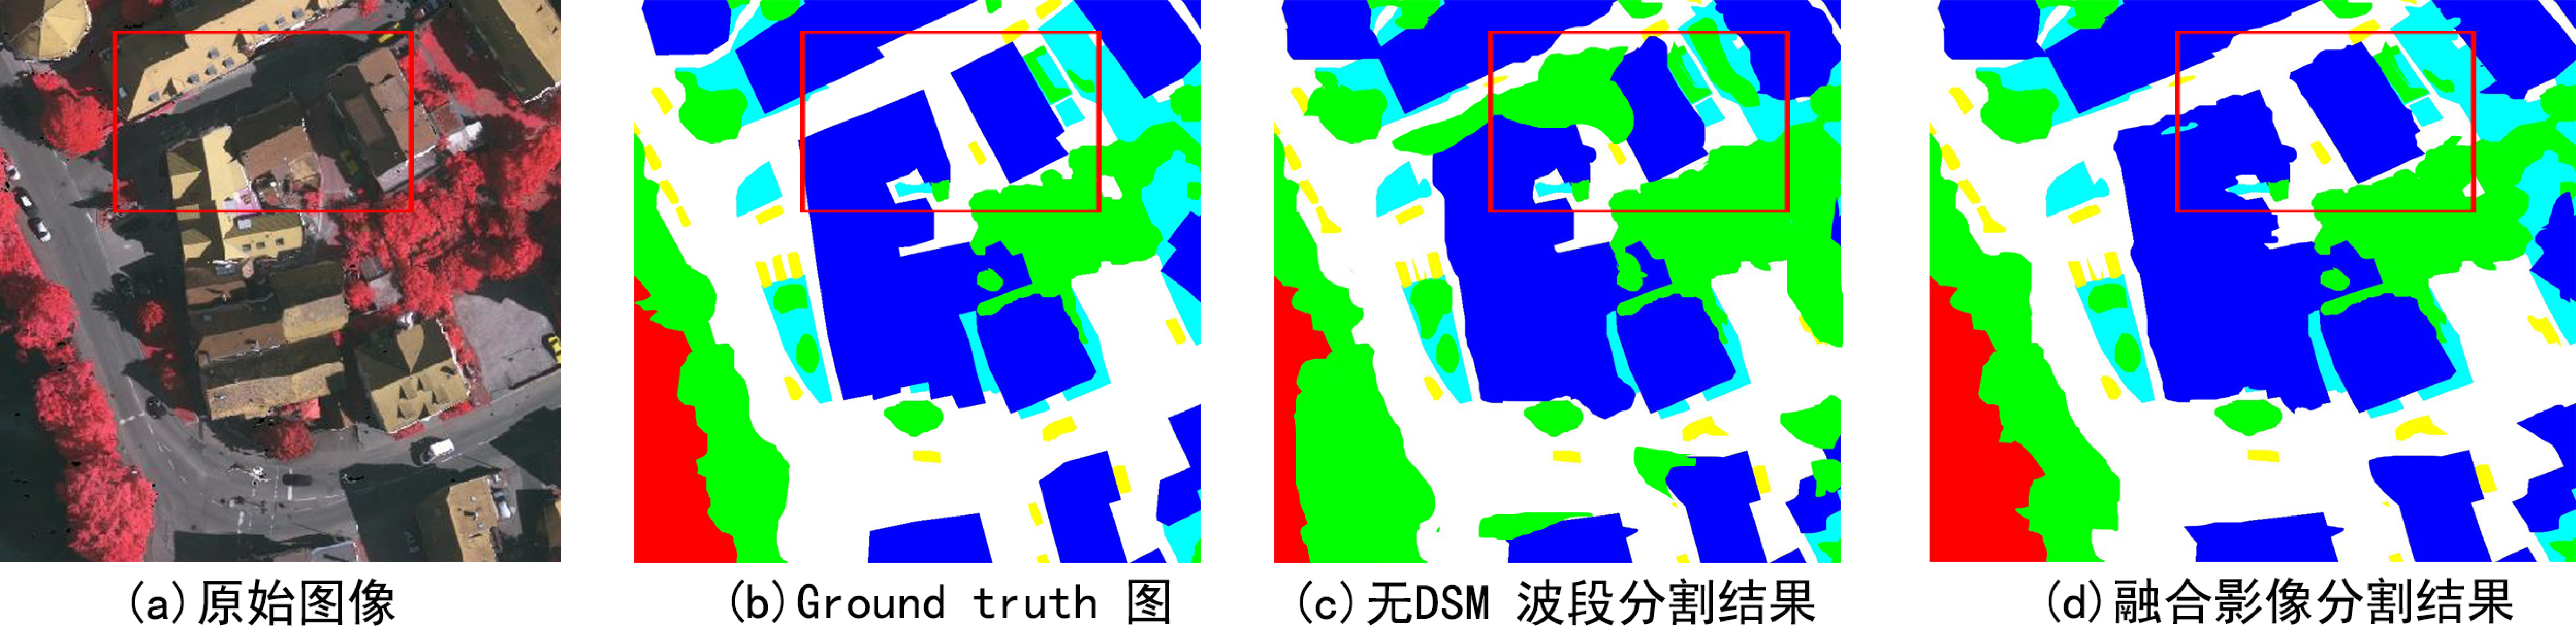
\includegraphics[width=0.9\textwidth]{figures/dsm_affect}
  \caption{DSM 波段对影像分类结果的影响}\label{fig:dsm_affect}
\end{figure}

文中使用的训练样本为三波段正射影像与一波段DSM 的融合数据。下文实验比较了DSM 数据对实验结果的影响。DSM 数据包含地形和地物高度等相关高程信息,“道路”、“低矮植被”和“建筑物”容易受不同地形、高度变化导致地物的特征起伏变化打,融合DSM 特征后更利于区分这些地物。图\ref{fig:dsm_affect} 中比较了正射影像是否融合DSM 数据对分割结果的影响。如图中红框区域为“建筑物”与“地面阴影”交叉部分,没有DSM 高程数据的分割模型中,将部分“阴影”了别错分为“树木”类别,同时,“建筑物”类别的边界也不完整。融合影像输入数据的分割结果则较好地解决了受高度特征影响的地物错分问题,尽可能保证“建筑物”边界的明确和完整。表\ref{tab:dsm_affect} 则统计了有无DSM 波段的数据源对实验分类精度的影响,通过对五类地物的分类精度、OA和mIoU 指标的对比,我实验返现输入数据加入DSM 波段后,“低矮植被”的分类精度提升最大,相比初始的$72.68\%$ 提升了$1.72\%$,达到$82.40\%$。整体的分类精度也由$79.52\%$ 提升到$80.15\%$。因此,融合DSM 高程信息数据能得到更优秀的分类精度和分割效果。

\begin{table}[htbp]
  \caption{DSM 波段对分类精度的影响}\label{tab:dsm_affect}
  \centering
  \begin{tabular}{ccccccccc}
    \toprule
   数据源             & 地面 & 低矮植被 & 树木 & 建筑物 & 车辆 & OA & mIoU \\
    \midrule
    正射影像     & $83.27\%$ & $72.68\%$ & $82.61\%$ & $86.33\%$ & $78.20\%$   & $79.52\%$ & $60.96\%$ \\
    正射影像+DSM & $83.78\%$ & $74.47\%$ & $82.40\%$ & $87.64\%$ & $78.83\%$ & $80.15\%$ & \textbf{$61.83\%$} \\
    \bottomrule
  \end{tabular}
\end{table}

\section{本章小结}
\label{sec:forth}
高分影像固有的不确定性和复杂的类内特征使得地物边界难以区分且同类别像素点难以保持空间一致性。此外,FCN 分类方法上采样操作会损失影像的特征细节,导致遥感影像地物边界更加难以正确识别。本章提出基于CGAN 的影像分类方法将生成对抗网络的思想应用到全卷积分割模型中,CGAN 网络对抗损失提升影像远距离像素点间类别标签的连续性,因而影像分类结果同类别像素点更具有一致性。对抗框架下分割模型的建模能力更强,一定程度上能提升分类精度。将文中提出的基于CGAN 的影像分类方法应用到Vaihingen 影像数据分割实验上,分割结果和分类精度均表明文中提出的方法整体上相比经典FCN 语义分割方法有着更优秀的分类效果。此外,文中实验结果也证明了融合DSM 波段高程信息的影像数据,可以进一步提升识别特征相近的不同地物类别的能力。
